\chapter{Introduzione a Kitten}\label{ch:kitten}
\begin{center}

\includegraphics[width=7cm]{cat4.jpg}
\end{center}
%
Kitten \`e il linguaggio di programmazione per il quale descriveremo in questo libro
un compilatore scritto in Java.
Bench\'e quindi questo libro non sia centrato solo su
Kitten, \`e necessario comunque cominciare a
prendere familiarit\`a con tale linguaggio, in modo da essere
coscienti di quello che \`e lo scopo del nostro compilatore.
Il fine di questo capitolo \`e di descrivere l'installazione del compilatore
Kitten e il linguaggio Kitten stesso. Il compilatore ci permetter\`a di
compilare ed eseguire tutti i programmi Kitten
di esempio che incontreremo in queste pagine.

Kitten \e un semplice linguaggio di programmazione imperativo a oggetti.
\E un linguaggio \emph{imperativo} \poiche
l'esecuzione dei programmi Kitten consiste in una sequenza di passi
specificati da \emph{comandi} e ciascun comando determina una modifica
dello stato dell'esecutore. \E un linguaggio \emph{a oggetti} \poiche
lo stato dell'esecutore lega le variabili del programma a degli \emph{oggetti}
appunto, \cioe zone di memoria con una propria identit\`a,
contenenti informazioni e che reagiscono
all'invocazione di \emph{metodi}. Va detto che Kitten non \`e un linguaggio
a oggetti \emph{puro}, nel senso che alcune variabili possono non essere legate
a oggetti, ma piuttosto a \emph{valori primitivi}. Esempi di valori primitivi
sono gli interi e i numeri in virgola mobile. Esistono pochissimi linguaggi di
programmazione puramente a oggetti. In particolare, va ricordato
Smalltalk~\cite{GoldbergR89}. Java~\cite{GoslingJSB05}
non \`e puramente a oggetti, perch\'e anch'esso ha dei tipi primitivi
(che per\`o coesistono con
delle versioni a oggetti dei tipi primitivi, \cioe le \emph{classi
involucro} tipo \texttt{java.lang.Integer} e simili).
Il motivo per cui i linguaggi a oggetti tendono a non essere puri
\`e che i valori primitivi sono gestibili molto pi\`u efficientemente
che gli oggetti e che per essi la semantica intesa dai programmatori
sarebbe difficilmente compatibile con la condivisione del valore fra pi\`u
variabili (\emph{aliasing}).

Possiamo immaginare Kitten come una versione semplificata di Java,
sia da un punto di vista sintattico che semantico. Lo scopo di Kitten \e
infatti quello di essere un linguaggio abbastanza semplice da potere essere
compilato ed eseguito senza eccessive complicazioni, ma al contempo
sufficientemente rappresentativo dei problemi che si presentano nella
compilazione dei linguaggi di programmazione attuali tipo Java.
In Kitten mancano all'appello aspetti \emph{secondari} di Java, come
\emph{i modificatori di visibilit\`a} (\texttt{public}, \texttt{protected},
\texttt{private}), i metodi e i campi \texttt{static}, le classi
astratte e le interfacce, le classi interne e quelle anonime,
i package, i campi costanti, le eccezioni e i finalizzatori.

\greycomment{Lo studente potrebbe domandarsi perch\'e non si \`e scelto
Java come linguaggio da compilare, al posto di Kitten. In fin dei conti,
Kitten non \`e utilizzato se non in questo corso e quindi la sua importanza
decade con il corso stesso. Il motivo \`e che la compilazione di Java
\`e estremamente complessa per essere descritta in un breve corso
di compilazione essendo Java, come abbiamo visto, molto pi\`u complicato
di Kitten. \`E invece pi\`u interessante chiedersi perch\'e non si
sia scritto un compilatore Kitten \emph{in Kitten}. Questo ci avrebbe
permesso, per esempio, di compilare il nostro compilatore con se stesso!
Il motivo questa volta \`e che Kitten \`e troppo povero per permettere
la definizione di un compilatore senza eccessivi sforzi di programmazione.
Per esempio, l'assenza dei modificatori di visibilit\`a e
del \emph{constructor chaining} priva la gerarchia delle classi di
ogni potere di incapsulazione, aprendo la strada a codice criptico
e scarsamente controllabile.
L'assenza dei package impedisce ogni strutturazione del progetto.
Va inoltre ricordato che esistono e che utilizzeremo degli
strumenti di sviluppo di compilatori scritti in Java, come JLex
(Capitolo~\ref{chap:lexical}) e JavaCup
(Capitolo~\ref{chap:syntactical}), e che tali strumenti andrebbero riscritti
ex-novo in Kitten.}
%
\section{Il compilatore Kitten}\label{sec:kitten_compiler}
%
Il compilatore Kitten \e scritto in Java. Si tratta di
uno strumento che permette di compilare dei sorgenti Kitten trasformandoli
in file \texttt{.class} eseguibili da una qualsiasi Java virtual machine.
Conseguentemente, sia il compilatore Kitten che il risultato della
compilazione dei sorgenti Kitten possono essere eseguiti su qualsiasi
architettura e sistema operativo, \purche sia installato un compilatore
e interprete Java. Le istruzioni che seguono descrivono l'installazione,
la compilazione e l'esecuzione del compilatore Kitten all'interno dell'ambiente
di sviluppo integrato Eclipse. Si assume che Eclipse contenga il modulo per
la gestione degli script Ant. Le istruzioni dovrebbero quindi essere eseguibili
su qualsiasi sistema operativo, anche se nel seguito mostreremo le istruzioni
per una shell di linux.

\begin{figure}[t]
\begin{verbatim}
                            class Miao {
                              method void main() {
                                "miao\n".output()
                              }
                            }
\end{verbatim}
\caption{Un programma Kitten che stampa una stringa e termina.}
  \label{fig:miao}
\end{figure}

La prima operazione da effettuare \`e di clonare il repository del compilatore Kitten,
tramite il programma git di gestione delle versioni. Ci si sposti nel workspace
di Eclipse e sia cloni il repository col comando:
%
\begin{verbatim}
git clone https://github.com/HotMoka/Kitten.git
\end{verbatim}
%
Verr\`a creata una directory di nome \texttt{Kitten}.
Si lanci quindi Eclipse e si crei un nuovo progetto Java,
di nome \texttt{Kitten}. Eclipse dovrebbe automaticamente riconoscere la presenza del progetto
e permetterne la compilazione o compilarlo automaticamente se la relativa opzioni \`e stata
attivata.

\javatip{Come sempre con \texttt{git}, \`e possibile aggiornare il compilatore alle
versioni successive che verranno prodotte, probabilmente pi\`u semplificate o debuggate.
A tal fine, basta spostarsi dentro il progetto Eclipse \texttt{Kitten} \`e invocare il comando
\texttt{git pull}.}

\noindent
A questo punto si apra la vista di Ant di Eclipse
(Window $\rightarrow$ Show View $\rightarrow$ Other\ldots e si selezioni Ant).
Quindi si selezioni il file \texttt{build.xml} col tasto sinistro del mouse e lo si trascini
sulla vista di Ant. Dovrebbe apparire la lista di task di Ant mostrata in Figura~\ref{fig:ant_tasks}.
Si faccia doppio click sul task di default \texttt{run-compiled-code}. Nella finestra della console
si dovrebbe assistere alla compilazione del compilatore e alla sua esecuzione su un file
Kitten di esempio, chiamato \texttt{Miao.kit}:

\begin{verbatim}
Buildfile: .../Kitten/build.xml
clean-bin: ...
generate-lexical-analyzer: ...
compile-lexical-analyzer: ...
generate-syntactical-analyzer: ...
compile-syntactical-analyzer: ...
compile-semantical-analyzer: ...
compile-kitten-bytecode-generator: ...
compile-java-bytecode-generator: ...
run-java-bytecode-generator: ...
     [java] Parsing and type-checking completed                 [51ms]
     [java] Translation into Kitten bytecode completed          [5ms]
     [java] Kitten bytecode dumping in dot format completed     [1ms]
     [java] Java bytecode generation completed                  [79ms]
     [java] Total compilation time was 135ms
run-compiled-code:
     [java] miao
\end{verbatim}

\noindent
Le ultime due righe sono per adesso le pi\`u interessanti. Esse indicano che l'esecuzione del
programma di esempio ha portato alla stampa della stringa \texttt{miao}. Quindi il programma
ha terminato la sua esecuzione.

\begin{figure}[t]
\begin{center}
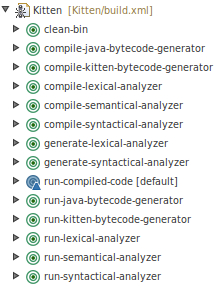
\includegraphics[width=5cm, height = 7cm]{pictures/ant_tasks.jpg}
\end{center}
\caption{I task di Ant per la compilazione e l'esecuzione del compilatore Kitten.}
\label{fig:ant_tasks}
\end{figure}
%
\section{Il nostro primo programma Kitten}\label{sec:first_kitten_programme}
%
La Figura~\ref{fig:miao} mostra il codice sorgente del programma
di esempio Kitten compilato ed eseguito nella sezione precedente. Si tratta
di un programma che stampa a video la
stringa \texttt{miao}, seguita da un ritorno carrello.
Si assume di avere inserito il programma
in Figura~\ref{fig:miao} dentro a un file testo di nome
\texttt{Miao.kit} che si trova nella sottodirectory
\texttt{testcases} del progetto Eclipse.
La sottodirectory \texttt{testcases} \e quella che utilizzeremo
per i nostri esperimenti, in modo da non sporcare la directory
principale di Kitten. Essa non ha comunque nulla di speciale:
potevamo scegliere un qualsiasi altro nome. \E invece importante
che il nome del file \texttt{Miao.kit} termini col suffisso \texttt{.kit}.
In caso contrario tale file non verr\`a riconosciuto dal compilatore
come un sorgente Kitten. La specifica del programma Kitten che
intendiamo compilare avviene tramite una propriet\`a nel file
\texttt{build.properties}:
%
\begin{verbatim}
kitten.example = Miao
\end{verbatim}
%
In futuro, occorrer\`a modificare tale propriet\`a per specificare un
altro file Kitten da compilare.

Ritorniamo un attimo all'output che ci \e stato stampato sulla console:
%
\begin{verbatim}
     [java] Parsing and type-checking completed                 [51ms]
     [java] Translation into Kitten bytecode completed          [5ms]
     [java] Kitten bytecode dumping in dot format completed     [1ms]
     [java] Java bytecode generation completed                  [79ms]
     [java] Total compilation time was 135ms
\end{verbatim}
%
La prima riga ci informa che Kitten ha effettuato un'analisi sintattica
(\emph{parsing}) sul file \texttt{Miao.kit}, al fine di garantire che non
contenga errori di sintassi. A questa fase ne \`e seguita una di verifica
semantica (\emph{type-checking}). Il tutto ha richiesto $51$ millisecondi.
A queste due fasi ne \`e seguita una in cui il nostro programma \`e
stato tradotto in un linguaggio chiamato \emph{Kitten bytecode}. Si tratta
di un linguaggio ispirato al Java bytecode ma molto pi\`u semplice di esso,
sul quale \`e per esempio possibile
ragionare per effettuare eventuali ottimizzazioni. Tale bytecode \`e
stato anche salvato su disco in formato \texttt{dot}, un
formato di descrizione di grafi che ci permette di visionare il risultato
di questa fase della compilazione. Infine, il Kitten bytecode \`e stato
tradotto in Java bytecode e salvato dentro \texttt{Miao.class},
che \`e proprio quello che alla fine \`e stato eseguito da Eclipse
con una Java virtual machine. Si noti che l'esecuzione di tale classe
pu\`o avvenire anche manualmente, fuori dal task Ant che ha compilato
il sorgente. Basta spostarsi dentro il progetto Eclipse ed eseguire:
%
\begin{verbatim}
java -cp bin:testcases Miao
\end{verbatim}
%
in cui la Java virtual machine \e stata eseguita fornendo come classpath
la directory \texttt{testcases} di \texttt{Miao.class} e la directory
\texttt{bin} in cui \e stata compilata la classe runtime
per le stringhe Kitten.

Sono tre i file che sono stati infatti compilati in Java
bytecode. Oltre a \texttt{Main.kit}, come ci aspettavamo, ci sono anche
\texttt{Object.kit} e \texttt{String.kit}. Questi sono due file Kitten
forniti insieme al compilatore. Il primo descrive la
classe \texttt{Object}, \cioe la superclasse di tutte le classi
Kitten. Esso \e stato compilato \poiche la classe \texttt{Miao.kit}
in Figura~\ref{fig:miao} estende (implicitamente) la classe
\texttt{Object.kit}. Il secondo descrive la classe delle stringhe.
Esso \e stato compilato \poiche il programma in Figura~\ref{fig:miao}
chiama il metodo \texttt{output()} sulle stringhe e tale metodo \e
definito proprio dentro \texttt{String.kit}.

Adesso che siamo riusciti a compilare ed eseguire un programma Kitten,
proviamo a guardarne \piu da vicino il sorgente in Figura~\ref{fig:miao}, per
iniziare a comprendere in cosa Kitten rassomigli a Java o si differenzi da esso.

La Figura~\ref{fig:miao} definisce una \emph{classe} Kitten di nome
\texttt{Miao}, \cioe una
matrice che pu\`o essere usata per generare degli \emph{oggetti} di tale
classe. Tali oggetti sono detti \emph{istanze} della classe.
Una classe pu\`o avere dei \emph{costruttori} che specificano come
generare degli oggetti di tale classe. Serve almeno un costruttore
per potere creare istanze di una classe. Dal momento che nessun costruttore
\`e presente in Figura~\ref{fig:miao}, nessuna istanza della classe
\texttt{Miao.kit} pu\`o essere creata.
Una classe pu\`o anche avere
dei \emph{metodi}, \cioe del codice etichettato con un nome che viene
eseguito al momento dell'\emph{invocazione} del metodo.
Fin qui ci sono solo somiglianze con Java.
Guardando attentamente la Figura~\ref{fig:miao},
notiamo per\`o anche molte differenze con Java. Per esempio, i metodi
sono introdotti dalle parole chiave \texttt{method}.
Inoltre, il punto e virgola, che in Java \e un \emph{terminatore} di comandi,
in Kitten \e invece un \emph{separatore} di comandi. Conseguentemente,
non si deve mettere alcun punto e virgola alla fine del metodo
\texttt{main} in Figura~\ref{fig:miao}. Inoltre, va osservato che non
ci sono costruttori di default in Kitten e che quindi una classe \emph{deve}
avere almeno un costruttore esplicito per potere essere
istanziata. Su tali istanze si possono poi chiamare i metodi
della classe. Fa eccezione il metodo \texttt{main}, che pu\`o essere
chiamato senza avere a disposizione alcuna istanza della classe.
Il metodo \texttt{main}, senza parametri e con tipo di ritorno \texttt{void},
\e in effetti quello che viene eseguito quando si esegue un programma Kitten.
Al momento dell'invocazione di tale metodo, non esiste ancora alcuna
istanza della classe.
%
\greycomment{
Si pu\`o dire, con terminologia presa in prestito da Java, che il metodo
\texttt{main} di Kitten \`e \textit{statico}, cio\`e invocato sulla classe
piuttosto che sulle istanze della classe. Si noti che esso \`e per\`o
l'unico metodo Kitten ad avere tale caratteristica: in Kitten non esiste
modo di dichiarare i metodi come \textit{statici}. Essi saranno sempre
implicitamente non \textit{statici}.}
%
\begin{figure}[t]
\begin{verbatim}
              class Fibonacci {
                constructor() {}

                method int fib(int n)
                  if (n = 0 | n = 1) then return 1
                  else return this.fib(n - 1) + this.fib(n - 2)

                method void main() {
                  String s := new String();
                  "Insert a relatively small number: ".output();
                  s.input();
                  "Fibonacci(".concat(s).concat(") = ".concat
                    (new Fibonacci().fib(s.toInt()))).output();
                  "\n".output()
                }
              }
\end{verbatim}
\caption{La funzione di Fibonacci in Kitten.}\label{fig:fibonacci}
\end{figure}
%
\section{Un esempio \piu complesso}\label{sec:fibonacci}
%
Si consideri il programma in Figura~\ref{fig:fibonacci}. Assumiamo che esso
sia scritto all'interno di un file testo di nome \texttt{Fibonacci.kit}.
Il suo metodo \texttt{main} chiede all'utente di immettere un numero intero
(positivo) \texttt{s} e quindi stampa l'\texttt{s}-esimo numero di Fibonacci.
Si noti che \texttt{s} \e una stringa, e che \e possibile leggere l'input da
tastiera e memorizzarlo dentro a una stringa tramite il metodo
\texttt{input()} della classe \texttt{String.kit}. Va osservato che, come
per tutte le invocazioni di metodo, la variabile \texttt{s} deve contenere
un oggetto affinch\'e su di essa si possa chiamare
il metodo \texttt{input()}; essa non deve contenere \texttt{nil}, pena
un errore a tempo di esecuzione del programma.
Sulle stringhe \e disponibile anche il metodo \texttt{toInt()} che trasforma
la stringa nell'intero corrispondente, se possibile. Esiste anche il metodo
\texttt{concat()} che restituisce la concatenazione di due stringhe o di
una stringa con un intero. Tutti questi metodi sono stati usati in
Figura~\ref{fig:fibonacci}. La Figura~\ref{fig:string} descrive tutti i
metodi della classe Kitten \texttt{String.kit}.
%
\begin{figure}[t]
\begin{center}
\begin{tabular}{|l|l|}
\hline
$s$\texttt{.length()} & restituisce la lunghezza (numero di caratteri) della
                        stringa $s$ \\
\hline
$s$\texttt{.toInt()} & restituisce l'intero rappresentato dalla stringa $s$; \\
                     & restituisce $0$ se $s$ non rappresenta un intero \\
\hline
$s$\texttt{.toFloat()} & restituisce il float rappresentato dalla stringa
                         $s$; \\
                       & restituisce $0.0$ se $s$ non rappresenta un float \\
\hline
$s$\texttt{.equals(}$s'$\texttt{)} & restituisce \textit{true} se e solo se
                                     le stringhe $s$ ed $s'$ \\
                                   & sono sintatticamente identiche \\
\hline
$s$\texttt{.input()} & memorizza dentro la stringa $s$ una sequenza di \\
                     & caratteri letti da tastiera fino al primo newline
                       (escluso) \\
\hline
$s$\texttt{.output()} & stampa a video la stringa $s$ \\
\hline
$s$\texttt{.concat(X)} & restituisce la concatenazione della stringa $s$ \\
                       & con $X$, che pu\`o essere un'altra stringa,
                         un intero, \\
                       & un float o un booleano. \Nec $s$ \nec $X$ sono
                         modificati \\
\hline
\end{tabular}
\end{center}
\caption{I metodi della classe Kitten \texttt{String.kit}.}
  \label{fig:string}
\end{figure}
%

La Figura~\ref{fig:fibonacci} mostra come sia possibile creare un
\emph{oggetto} tramite l'espressione \texttt{new}. Esattamente come
in Java, tale istruzione chiama il corrispondente costruttore della
classe, in questo caso il costruttore di \texttt{Fibonacci}
e quello di \texttt{String.kit} senza
parametri. La stessa figura mostra come sia possibile definire un
metodo ricorsivo \texttt{fib}. Si noti che, a differenza di Java, non
\e possibile lasciare sottinteso il riferimento \texttt{this} quando
si chiama un metodo sull'oggetto corrente (o se ne modifica un campo).
Si noti infine che la disgiunzione di due condizioni booleane si
ottiene con la barretta \texttt{|} e che nel comando
condizionale \e obbligatorio
usare la parola chiave \texttt{then}, che \e invece sottintesa in C e Java.
%
\section{Le diverse compilazioni del compilatore Kitten}
  \label{sec:kitten_compilations}
%
Nella Sezione~\ref{sec:kitten_compiler} abbiamo usato il comando
\texttt{make generatejb} per compilare il compilatore Kitten. Tale comando
esegue una sequenza di comandi di compilazione specificati dentro al file
\texttt{makefile} e il cui risultato \`e la compilazione del compilatore
Kitten in modo che esso possa poi
generare il Java bytecode dei file sorgenti. Esistono
altri modi per compilare il compilatore Kitten, in modo da attivare \piu o
meno fasi della compilazione. Esse sono le seguenti:
%
\begin{description}
\item[\texttt{make lexical}:]
  Compila il compilatore Kitten in modo che esso esegua
  la sola analisi lessicale
  del sorgente da compilare (Capitolo~\ref{chap:lexical});
\item[\texttt{make syntactical}:]
  Compila il compilatore Kitten in modo che esso esegua
  le sole analisi lessicale
  e sintattica (Capitolo~\ref{chap:syntactical}) del sorgente da compilare;
\item[\texttt{make semantical}:]
  Compila il compilatore Kitten in modo da eseguire solo le analisi lessicale,
  sintattica e semantica (o type-checking,
  Capitolo~\ref{chap:semantical}) del sorgente da compilare;
\item[\texttt{make translate}:]
  Compila il compilatore Kitten in modo da eseguire solo le analisi lessicale,
  sintattica e semantica del sorgente da compilare e la generazione del
  codice intermedio Kitten bytecode
  (Capitolo~\ref{chap:translate});
\item[\texttt{make generatejb}:]
  Compila il compilatore Kitten in modo da eseguire solo le analisi lessicale,
  sintattica e semantica del sorgente da compilare, la generazione del codice
  intermedio Kitten bytecode e la sua trasformazione nel codice eseguibile
  Java bytecode (Capitolo~\ref{chap:translate});
\item[\texttt{make analyse}:]
  Compila il compilatore Kitten in modo da eseguire le analisi lessicale,
  sintattica e semantica del sorgente da compilare, la generazione del codice
  intermedio Kitten bytecode, alcune sue analisi statiche
  e la sua trasformazione nel codice eseguibile
  Java bytecode (Capitolo~\ref{chap:analyse}).
\end{description}
%
\greycomment{Si noti che solo le due ultime modalit\`a di compilazione
generano un compilatore Kitten il quale a sua volta genera dei file eseguibili
\texttt{.class} scritti in Java bytecode. Non c`\`e quindi da meravigliarsi
se dopo un \texttt{make syntactical} il comando \texttt{./run} non funzioni
o esegua una vecchia versione del programma che si vuole eseguire:
a quel punto, il compilatore Kitten non genera pi\`u alcun file
\texttt{.class} eseguibile. \`E necessario eseguire nuovamente un
\texttt{make generatejb} oppure un \texttt{make analyse} per ottenere
un compilatore Kitten che genera file \texttt{.class} eseguibili.}

Altri comandi \texttt{make} effettuano operazioni
di pulizia o documentazione del codice:
%
\begin{description}
\item[\texttt{make clean}:]
  Pulisce le directory dell'installazione Kitten, eliminando file temporanei
  di \texttt{emacs}, i file \texttt{.class} di Java e file \texttt{dot}
  generati dentro la directory \texttt{testcases};
\item[\texttt{make javadocs}:]
  Rigenera la documentazione JavaDoc del compilatore Kitten.
  Tale documentazione viene scritta dentro la directory
  \texttt{javadocs} ed \`e consultabile con un qualsiasi browser
  internet a partire dal file \texttt{index.html}.
\end{description}
%
\javatip{Ci si abitui subito a consultare tale documentazione. Per
esempio, si inserisca una url del tipo
\texttt{file:///home/spoto/kitten\_XXX/javadocs/index.html}
dentro un browser internet. Ovviamente dovrete usare un nome di directory
corrispondente al vostro punto di installazione del compilatore Kitten
e alla struttura del vostro file system.
Dovreste poter vedere l'elenco di tutti i package e di tutte le classi
che compongono il compilatore Kitten, e consultare la documentazione
dei loro campi e
metodi. Usare tale documentazione facilita estremamente lo sviluppo di
modifiche del compilatore Kitten, come per esempio
eventuali progetti assegnati allo studente.}

Adesso che abbiamo capito come installare e compilare il compilatore
Kitten e come usarlo per compilare file scritti nel linguaggio Kitten,
diamo un'occhiata pi\`u da vicino alla struttura e al funzionamento di
tale linguaggio.
%
\section{Comandi Kitten}\label{sec:commands}
%
Un \emph{comando} \e una porzione di codice Kitten la cui esecuzione
pu\`o modificare lo stato dell'esecutore ma non fornisce alcun valore.
Il concetto di \emph{stato} va preso nel senso \piu
generale possibile: esso include l'insieme delle variabili del programma,
il loro tipo e valore, ma anche il contenuto del video.
Per esempio, la Figura~\ref{fig:miao} contiene il
comando \verb|"miao\n".output()|, il cui effetto \e di stampare su video
la stringa \texttt{miao} seguita da un carattere di newline.
Un altro esempio di comando Kitten \e \verb|int y := 0|, che \emph{dichiara}
una variabile di nome \texttt{y}, di tipo \texttt{int} e con valore iniziale
pari a $0$.

I comandi Kitten
possono essere \emph{composti}. Per esempio, se abbiamo due comandi
$c_1$ e $c_2$, possiamo comporli sequenzialmente
scrivendo $c_1;c_2$. Quello che otteniamo
\e ancora un comando, la cui esecuzione consiste nell'esecuzione di $c_1$
seguita dall'esecuzione di $c_2$. Per esempio, scrivendo
\verb|"hello".output(); " kitten".output()| otteniamo l'effetto di
stampare su video la stringa \texttt{hello kitten}. Oltre a questa
composizione sequenziale di comandi, Kitten fornisce delle forme
standard di composizione di comandi che si trovano in tantissimi altri
linguaggi. Per esempio, il \emph{condizionale}
\texttt{if (y >= 18) then }$c_1$\texttt{ else }$c_2$
\e un comando che esegue $c_1$ se la variabile \texttt{y} contiene un valore
maggiore o uguale a $18$ ed esegue $c_2$ altrimenti. Se quindi scriviamo
%
\begin{verbatim}
  if (y >= 18) then "man".output()
               else "kid".output()
\end{verbatim}
%
otteniamo di stampare la stringa \texttt{man} se la variabile \texttt{y}
contiene un valore maggiore o uguale a $18$, e di stampare
\texttt{kid} altrimenti.
Si noti che, essendo in Kitten il punto e virgola un separatore di comandi,
non dobbiamo inserirlo dopo il comando \verb|"man".output()|.

Si faccia attenzione adesso al seguente codice:
%
\begin{verbatim}
  if (y >= 18) then "old ".output(); "man".output()
               else "kid".output()
\end{verbatim}
%
L'intenzione del programmatore era quella di stampare la stringa
\texttt{old man} se la variabile \texttt{y} contiene un valore maggiore o
uguale a $18$, e di stampare \texttt{kid} altrimenti. Purtroppo il compilatore
Kitten non ama tale codice, e segnala un errore di sintassi in corrispondenza
all'\texttt{else}. Il motivo \e che esso interpreta tale codice come
un comando \verb|if (y >= 18) then "old ".output()| seguito da
un secondo comando \verb|"man".output()| seguito a sua volta
da uno stranissimo comando
\verb|else "kid".output()| e non trova neppure il punto e virgola che
dovrebbe separare i comandi in Kitten. La giusta sintassi sarebbe stata
invece la seguente:
%
\begin{verbatim}
  if (y >= 18) then { "old ".output(); "man".output() }
               else "kid".output()
\end{verbatim}
%
Questo codice viene accettato e compilato dal compilatore Kitten ed esegue
esattamente quello che il programmatore aveva in mente. Le parentesi
graffe sono un ulteriore costrutto di composizione di comandi. Se abbiamo
un comando $c$, allora la notazione \texttt{\{}$c$\texttt{\}} \e ancora
un comando, la cui esecuzione \e semplicemente l'esecuzione di $c$.
Tale costrutto permette in pratica di raggruppare una sequenza di comandi
per formare un comando unico di cui si specifica l'inizio e la fine, come
nell'esempio precedente. Deve essere
chiaro comunque che del codice fra parentesi graffe \emph{\`e} un comando.
Possiamo quindi dire che la parola chiave \texttt{then} \e sempre seguita
da uno \emph{e un solo}
comando (non da uno \emph{o \piu} comandi). Similmente, in Kitten
il corpo di un metodo o costruttore \e sempre \emph{un} comando. Per esempio,
in Figura~\ref{fig:fibonacci} il corpo del costruttore vuoto \e il
\emph{comando vuoto} \verb|{}|, la cui esecuzione lascia lo stato immutato.
Il corpo del metodo \texttt{main} in Figura~\ref{fig:miao}
\e il comando \verb|{ "miao\n".output() }|,
che potrebbe essere semplificato in \verb|"miao\n".output()|. In pratica,
useremo le parentesi graffe solo se il corpo di un metodo o costruttore
\e \cosi esteso che abbiamo bisogno di dividerlo in \piu comandi in sequenza,
come accadr\`a in tantissimi casi.
%
\greycomment{Si noti che in C o Java le parentesi
graffe sono ugualmente un costrutto per ottenere
un comando composto, ma sono in alcuni casi
obbligatorie dove Kitten potrebbe non richiederle, come all'inizio del corpo
dei metodi e costruttori. Come abbiamo gi\`a detto, anche le regole di
uso del punto e virgola sono diverse fra Kitten (dove esso \`e un
\emph{separatore} di comandi) e C e Java (dove esso \`e un
\emph{terminatore} di comandi). Queste differenze, unitamente all'obbligo
in Kitten della parola chiave \texttt{then} nei condizio\-nali,
sono spesso all'origine di
\emph{misteriosi} messaggi di errore emessi dal compilatore Kitten e che
lasciano perplessi non pochi studenti.}
%
\section{Valori Kitten}\label{sec:values}
%
Abbiamo detto all'inizio della Sezione~\ref{sec:commands} che l'esecuzione
di un comando non fornisce alcun \emph{valore}. Ma cos'\e un valore?
Possiamo definirlo come un pezzo di informazione contenuto nella memoria
del calcolatore. I valori possono essere creati, legati a variabili del
programma, copiati, condivisi, modificati e confrontati.

Kitten gestisce i seguenti valori:
%
\begin{itemize}
\item valori \emph{primitivi}, non creabili, n\'e modificabili,
      n\'e condivisibili:
      \begin{itemize}
      \item i numeri interi: $\ldots,-5,-4,-3,-2,-1,0,1,2,3,4,5,\ldots$;
      \item i numeri in virgola mobile a singola precisione:
            $3.14, -1.13,\ldots$;
      \item i booleani \textit{true} e \textit{false};
      \item il riferimento \textit{nil};
      \end{itemize}
\item valori \emph{non primitivi} o \emph{riferimento},
      creabili, modificabili e condivisibili:
      \begin{itemize}
      \item gli \emph{oggetti}, \cioe delle zone di memoria divisibili in
            varie sotto-zone chiamate \emph{campi} o \emph{variabili
            d'istanza}
            dell'oggetto. I campi contengono a loro volta dei valori.
            La strutturazione in campi di un oggetto Kitten \`e descritta
            dalla \emph{classe} dell'oggetto, che in Kitten viene specificata
            al momento della crezione dell'oggetto stesso e non \`e pi\`u
            mutabile; diremo che un oggetto \`e un'\emph{istanza} della
            sua classe;
      \item gli \emph{array} o \emph{vettori}, \cioe delle zone di memoria
            divisibili in varie sotto-zone, chiamate \emph{elementi}
            dell'array e indirizzabili tramite un
            riferimento numerico intero non negativo.
            Gli elementi di un array contengono a loro
            volta dei valori. La strutturazione in elementi di un array,
            cio\`e il numero e il tipo degli elementi,
            viene specificata in Kitten al momento della sua creazione e dopo
            non \`e pi\`u mutabile.
      \end{itemize}
\end{itemize}
%
I valori esistono solo a tempo di esecuzione. Si badi quindi a non confondere
l'\emph{espressione sintattica} \texttt{2} in Figura~\ref{fig:fibonacci} con il
suo \emph{valore semantico} $2$ che essa assume a tempo di esecuzione. Nel
primo caso si tratta semplicemente di un carattere immesso dal programmatore
nel testo del programma. Nel secondo caso si tratta di un'entit\`a matematica,
il numero intero $2$ appunto. Questa distinzione \e ancora \piu chiara per
i valori non primitivi. Per esempio, l'espressione sintattica
\texttt{new String()} in Figura~\ref{fig:fibonacci} \e solo una sequenza
di caratteri digitati dal programmatore, il cui significato \e di creare
un oggetto di classe \texttt{String.kit} \emph{a tempo di esecuzione}.
In particolare, se la stessa espressione viene eseguita \piu volte,
essa crea \piu oggetti diversi della classe \texttt{String.kit}.
%
\greycomment{In genere, in un linguaggio di programmazione si distinguono
concetti relativi al momento della compilazione, come la sintassi delle
espressioni, e concetti relativi al momento dell'esecuzione del programma,
come il valore delle espressioni. Ritroveremo spesso questa distinzione in
futuro. Spesso indicheremo come \emph{statici} i primi e come \emph{dinamici}
i secondi.}

I valori possono essere \emph{legati} o \emph{copiati} dentro a una variabile
del programma. Per esempio, in Figura~\ref{fig:fibonacci}, l'oggetto creato
dall'espressione \texttt{new String()} viene memorizzato dentro alla variabile
\texttt{s}. Si noti che \texttt{s} non \e una stringa. Essa \e una variabile
che \emph{contiene} o \emph{fa riferimento} a un oggetto stringa.
Ci\`o nonostante, \`e convenzione comune
dire che \texttt{s} \emph{\e} un oggetto quando
si dovrebbe dire che \texttt{s} \emph{contiene} un oggetto. Ci adegueremo anche
noi a questo uso, ma deve essere chiara la distinzione fra variabile e
suo valore.

Il comando \texttt{s := new String()} in Figura~\ref{fig:fibonacci} \e
chiamato \emph{assegnamento}. Si noti l'uso di \texttt{:=} al posto del
solo \texttt{=} come si farebbe in C e Java. L'esecuzione di questo
assegnamento consiste nell'assegnare alla variabile \texttt{s} un riferimento
all'oggetto appena creato dall'espressione \texttt{new String()}.
Si noti che non \e l'oggetto che viene copiato, ma un suo riferimento,
esattamente come in Java. Per cui un successivo assegnamento
\texttt{s1 := s} avrebbe l'effetto di legare anche la variabile
\texttt{s1} allo \emph{stesso} oggetto a cui abbiamo appena legato
la variabile \texttt{s}. In questo caso di oggetto ne esiste uno solo,
raggiungibile sia tramite \texttt{s} che tramite \texttt{s1}. Diremo quindi
che tale oggetto \e \emph{condiviso} fra \texttt{s} ed \texttt{s1}.
Ogni modifica all'oggetto effettuata tramite \texttt{s} sar\`a automaticamente
visibile anche tramite \texttt{s1}.
La situazione \e ben diversa per i valori primitivi, che vengono sempre copiati
da un assegnamento. Per esempio, il comando
\texttt{i := 3; i1 := i} ha l'effetto di legare sia \texttt{i} che \texttt{i1}
allo stesso numero intero $3$, ma una successiva modifica di \texttt{i}
non influisce sul valore legato ad \texttt{i1}.
%
\section{Espressioni Kitten}\label{sec:expressions}
%
Un'\emph{espressione} \e un pezzo di codice Kitten la cui esecuzione,
detta \emph{valutazione},
pu\`o modificare lo stato dell'esecutore e, \emph{inoltre}, fornisce un
valore, chiamato appunto \emph{valore dell'espressione}. Per esempio, la
Figura~\ref{fig:miao} contiene l'espressione \verb|"miao\n"|. Il suo
valore \e un oggetto di tipo stringa che rappresenta la sequenza di
caratteri \texttt{m}-\texttt{i}-\texttt{a}-\texttt{o} seguita da un
carattere di newline. Un altro esempio \e \texttt{s} in
Figura~\ref{fig:fibonacci}.
Essa \e un'espressione il cui valore \e il contenuto della variabile
\texttt{s} in tale punto del programma.
Si potrebbe pensare che, in effetti, le espressioni
hanno un valore ma non modificano mai lo stato dell'esecutore.
Questo \e vero negli esempi fatti fin qui, ma in futuro vedremo
che anche la chiamata di un metodo pu\`o essere un'espressione, \purche
il metodo non abbia \texttt{void} come tipo di ritorno.
Il valore di una tale espressione \e infatti
il valore di ritorno del metodo. Un esempio \e l'espressione
\texttt{this.fib(n - 1)} in Figura~\ref{fig:fibonacci}. Dal momento che
il corpo del metodo chiamato pu\`o contenere comandi arbitrari,
dobbiamo ammettere che un'espressione Kitten possa modificare lo stato
dell'esecutore. In particolare, diremo che un'espressione contiene
un \emph{side-effect} o \emph{effetto di bordo} se la sua valutazione
modifica lo stato dell'esecutore. Altrimenti essa non contiene side-effect.
In Kitten l'unica espressione che pu\`o contenere side-effect \e la chiamata
di metodo. Altri linguaggi hanno altre espressioni con side-effect, come
i preincrementi e postincrementi di variabili numeriche in
linguaggi tipo C o Java: \texttt{i++}. Queste espressioni non esistono per\`o
in Kitten.

Anche le espressioni, come i comandi della Sezione~\ref{sec:commands},
sono definite in maniera ricorsiva. Conseguentemente, possiamo \emph{comporre}
espressioni complesse a partire da espressioni \piu semplici. Per esempio,
se abbiamo due espressioni $e_1$ ed $e_2$ allora possiamo comporle per
formare l'espressione $e_1$\texttt{-}\ $e_2$ la cui valutazione valuta
$e_1$, poi $e_2$ ed infine calcola la differenza del valore di $e_1$ meno
quello di $e_2$. Tale differenza \e il valore dell'espressione
$e_1$\texttt{-}\ $e_2$.
Un esempio \e l'espressione \texttt{n - 1} in Figura~\ref{fig:fibonacci}.

I mondi delle espressioni e dei comandi non sono separati ma strettamente
interdipendenti. Per esempio, il comando
\verb|"miao\n".output()| in Figura~\ref{fig:miao} \e costruito a partire
dall'espressione \verb|"miao\n"|. In generale, potremmo dire che il
comando \emph{chiamata di metodo} si costruisce a partire da espressioni
$e$, $e_1$, \ldots, $e_n$ con la sintassi
$e\mathtt{.m(}e_1,\ldots,e_n\mathtt{)}$, dove \texttt{m} \e il nome del
metodo che si intende chiamare \emph{sul} valore dell'espressione
$e$ \emph{con parametri} pari al valore delle espressioni $e_1,\ldots,e_n$.
Questo mostra che un comando Kitten pu\`o costruirsi a partire da espressioni
Kitten. Il viceversa non accade in Kitten, ma pu\`o accadere
in altri linguaggi. Per esempio, in C esiste
l'\emph{espressione virgola} $\mathtt{(}c\mathtt{,}e\mathtt{)}$ la cui
esecuzione esegue il comando $c$, valuta l'espressione $e$ e infine
ritorna il valore di $e$.
%
\section{Tipi Kitten}\label{sec:types}
%
Kitten \e un linguaggio di programmazione \emph{tipato}. Questo vuol dire
che i valori della Sezione~\ref{sec:values} sono organizzati in gruppi
detti appunto \emph{tipi}. I tipi specificano le operazioni che su tali
valori si possono effettuare. Per esempio, il tipo \texttt{int} raggruppa
i valori interi di Kitten. Su un valore di tipo intero, Kitten permette di
effettuare addizioni, sottrazioni, ecc. L'oggetto creato dall'espressione
\texttt{new String()} in Figura~\ref{fig:fibonacci} \e di tipo \texttt{String},
per cui su di esso \e possibile applicare tutti i metodi della
Figura~\ref{fig:string}. Non \e invece possibile applicare su di esso
addizioni o sottrazioni.

I tipi Kitten corrispondono ai gruppi di valori che abbiamo descritto
nella Sezione~\ref{sec:values}. In particolare, Kitten ha i tipi
\emph{primitivi} \texttt{int}, \texttt{float}, \texttt{boolean} e
\texttt{nil}, nonch\'e i tipi \emph{non primitivi} corrispondenti
a tutti i nomi delle classi che costituiscono il
programma (per gli oggetti) e al tipo
\texttt{array of} $t$ dove $t$ \e il tipo degli elementi dell'array.
L'insieme dei tipi Kitten \e parzialmente ordinato rispetto a una
\emph{relazione di sottotipaggio} $\le$ che esprime la \emph{compatibilit\`a}
fra tipi. Se $t_1\le t_2$ allora \e possibile utilizzare un valore del
tipo $t_1$ ogni volta che viene richiesto un valore di tipo $t_2$.
Per esempio, \`e possibile assegnare un valore di tipo $t_1$ a una
variabile dichiarata di tipo $t_2$, oppure passare tale valore come parametro
a un metodo che si aspettava un valore di tipo $t_2$.
La relazione $\le$ \`e formalmente definita come
la chiusura transitiva e riflessiva della seguente relazione:
%
\begin{eqnarray*}
  &\mathtt{int}\le\mathtt{float}\\
  &\kappa_1\le\kappa_2\quad\text{se la classe $\kappa_1$ estende la classe $\kappa_2$}\\
  &\mathtt{array\ of\ }t_1\le\mathtt{array\ of\ }t_2\quad
    \text{se $t_1\le t_2$ e $t_1$ non \e un tipo primitivo}\\
  &\mathtt{nil}\le\kappa\quad\text{per ogni classe $\kappa$}\\
  &\mathtt{nil}\le\mathtt{array\ of\ }t\quad\text{per ogni tipo $t$}\\
  &\mathtt{array\ of\ }t\le\mathtt{Object}\quad\text{per ogni tipo $t$.}
\end{eqnarray*}
%
Si noti che tale definizione implica che ogni array \`e un sottotipo
della classe \texttt{Object} e che
$\mathtt{array\ of\ int}\le\mathtt{array\ of\ int}$ (per riflessivit\`a).
Invece tale definizione implica che non \e vero che
$\mathtt{array\ of\ int}\le\mathtt{array\ of\ float}$, bench\'e
$\mathtt{int}\le\mathtt{float}$. La motivazione di questa non monotonia
nella relazione di sottotipaggio degli array sar\`a chiara in seguito.
Se $t_1\le t_2$ diremo che $t_1$ \e un \emph{sottotipo} di $t_2$ e che
$t_2$ \e un supertipo di $t_1$. Se $t_1\not=t_2$ scriveremo
$t_1<t_2$ e diremo che $t_1$ \`e un sottotipo \emph{stretto}
di $t_2$ e che $t_2$ \`e un supertipo \emph{stretto} di $t_1$.

Kitten \e un linguaggio di programmazione a \emph{tipaggio statico}.
Questo vuol dire che a ciascuna espressione che figura in un programma Kitten
viene associato un tipo \emph{al momento della compilazione}. Le regole che
specificano come questo tipo venga assegnato alle espressioni si chiamano
\emph{regole di tipaggio statico}. Lo strumento che effettua l'assegnazione
di un tipo a ciascuna espressione di un programma si chiama
\emph{analizzatore semantico} o \emph{type-checker}
del linguaggio (Capitolo~\ref{chap:semantical}). Per esempio, l'analizzatore
semantico di Kitten etichetta l'espressione \texttt{new String()} in
Figura~\ref{fig:fibonacci} con il tipo \texttt{String}. Esso inoltre
etichetta l'espressione \texttt{this.fib(n - 1)} con il tipo \texttt{int},
poich\'e il tipo di ritorno del metodo \texttt{fib} \`e \texttt{int}.
Molti linguaggi di programmazione di uso corrente hanno un tipaggio statico.
Per esempio C, C++ e Java. Diverso \`e il caso di un linguaggio tipo Prolog
e di alcuni dialetti del Basic,
in cui viene assegnato un tipo alle espressioni ma solo
\emph{a tempo di esecuzione}. In tal caso, si parla di un linguaggio di
programmazione a \emph{tipaggio dinamico}. Si noti che il tipaggio dinamico
permette a un'espressione di avere tipi diversi in tempi diversi, mentre
il tipaggio statico deve assegnare uno e un solo tipo a un'espressione.

Cosa abbiamo guadagnato ad avere un linguaggio a tipaggio statico piuttosto
che dina\-mico? Molto. In particolare, il tipaggio statico ci permette di
eseguire l'analisi semantica del programma solo una volta a tempo di
compilazione, piuttosto che in continuazione a tempo di esecuzione.
Il programma sar\`a quindi \piu veloce. Non solo. Il tipaggio dinamico richiede
di conoscere il tipo dei valori a tempo di esecuzione per potere
ricostruire quello delle espressioni. Per
esempio, qual \e il tipo dell'espressione \texttt{y} a tempo di esecuzione?
Occorre guardare cosa contiene \texttt{y} e capire di che tipo sia tale valore.
Ma un valore \`e, dal punto di vista del computer, semplicemente una sequenza
di bit. Due variabili \texttt{y} e \texttt{z} potrebbero contenere la
stessa rappresentazione binaria ma avere valori diversi \poiche una
andava pensata (ovvero, era stata dichiarata)
di tipo \texttt{int} e l'altra di tipo \texttt{float}.
Quello che manca \e un'indicazione esplicita del tipo del valore.
Ecco quindi che i linguaggi a tipaggio dinamico sono costretti
ad associare ai valori un'etichetta che specifica il tipo del valore.
Questa etichetta occupa spazio e rallenta l'esecuzione del programma.
La coppia valore pi\`u etichetta \e detta rappresentazione \emph{boxed} di
un valore. Il solo valore \e detto rappresentazione \emph{unboxed} di
se stesso. Potremmo quindi dire che in un linguaggio a tipaggio statico
\e sufficiente utilizzare una rappresentazione unboxed dei valori, il che
rende molto \piu semplice ed efficiente la sua implementazione rispetto
a un linguaggio a tipaggio dinamico, in cui \e obbligatoria la \piu pesante
rappresentazione boxed. Va detto comunque che i linguaggio
a tipaggio dinamico offrono maggiore flessibilit\`a al programmatore e sono
quindi spesso preferiti da chi lavora nell'ambito
dell'intelligenza artificiale. Infine, va osservato che nei linguaggi a
oggetti si \e comunque obbligati a usare una rappresentazione boxed per la
maggior parte degli oggetti (normalmente, per tutti gli oggetti),
anche se il linguaggio ha un tipaggio statico,
a causa della presenza di chiamate virtuali con late-binding
e di cast controllati a tempo di esecuzione. La rappresentazione unboxed
\e quindi limitata ai soli valori primitivi.

Kitten \e un linguaggio di programmazione \emph{fortemente tipato}.
Questo significa in primo luogo che esso \e tipato. Ma significa
anche che il tipo assegnato (a tempo di compilazione, nel caso di Kitten)
alle espressioni dall'analizzatore semantico
\e un supertipo di quello del valore delle stesse espressioni a tempo
di esecuzione. In altre parole, l'analizzatore semantico ha etichettato
\emph{bene}, senza \emph{sbagliare},
le espressioni del programma, in modo tale che il tipo scelto
\e corretto (un supertipo, appunto)
rispetto a quello che poi avranno tali espressioni quando andremo ad eseguire
il programma. Per esempio, il fatto che l'espressione \texttt{new String()} in
Figura~\ref{fig:fibonacci} sia stata etichettata con il tipo \texttt{String}
\e consistente con il fatto che, a tempo di esecuzione, tale espressione
avr\`a un valore di tipo \texttt{String}. Come Kitten,
anche il linguaggio Java \e
fortemente tipato. Mentre non sono fortemente tipati C, C++ o C\#, \poiche
\e possibile camuffare il tipo delle espressioni tramite cast non
controllati, ed \e anche possibile spacciare per oggetti puntatori a memoria
forgiati a partire da valori interi, o infine accedere a zone di memoria
oltre i limiti di un array senza garanzia che questo blocchi l'esecuzione
del programma e forgiando quindi \emph{valori} del tipo dell'array
a partire da configurazioni causali di bit.

Cosa abbiamo guadagnato dalla scelta di avere un linguaggio
\emph{fortemente} tipato piuttosto che semplicemente tipato? Anche in questo
caso abbiamo guadagnato molto. In particolare, abbiamo ottenuto la
possibilit\`a di garantire, a tempo di compilazione, che tutta una serie
di propriet\`a relative ai tipi dei valori delle espressioni saranno
sicuramente vere a tempo di esecuzione. Non servir\`a quindi verificarle
a tempo di esecuzione. Per esempio, si consideri l'espressione
\texttt{s} in Figura~\ref{fig:fibonacci}. Essa riceve dall'analizzatore
semantico il tipo \texttt{String}. \Poiche Kitten \e fortemente tipato,
sappiamo che a tempo di esecuzione dentro la variabile \texttt{s} troveremo
\emph{realmente}
un valore di tipo \texttt{String}. Conseguentemente, non occorre verificare,
a tempo di esecuzione, che l'oggetto contenuto dentro \texttt{s} abbia
effettivamente un metodo chiamato \texttt{input}, \perche tale controllo
\e superfluo, avendo \texttt{String} un metodo chiamato \texttt{input}.
In altre parole, un linguaggio a tipaggio forte ci permette di spostare
a tempo di compilazione un gran numero di controlli sulla consistenza
di quello che il programmatore ha scritto. Tali controlli devono invece
essere effettuati a tempo di esecuzione nel caso di un linguaggio a
tipaggio debole (\cioe non forte). Da un punto di vista di verifica del
software, possiamo dire che un linguaggio a tipaggio forte permette
all'analizzatore semantico di \emph{dimostrare} a tempo di compilazione
che nulla \emph{andr\`a storto}
a tempo di esecuzione, relativamente a una larga
classe di errori di tipo che include l'esistenza dei metodi al momento
della loro chiamata, la correttezza dei valori passati ai metodi,
la consistenza dei valori assegnati alle variabili, ecc. Ma non include
purtroppo
propriet\`a come la correttezza dei cast, la non-nullness dei ricevitori
delle chiamate di metodo e degli accessi ai campi e la legalit\`a
degli indici per l'accesso agli array. Tali propriet\`a
vengono normalmente verificate a tempo di esecuzione anche nei linguaggi
a tipaggio forte.

\greycomment{L'analizzatore semantico, che assegna un tipo statico alle
espressioni e garantisce la correttezza di comandi ed espressioni,
\`e spesso estremamente severo, al punto da vietare cose che apparentemente
sono giudicate \emph{corrette} da molti programmatori. Per esempio, se
\texttt{y} \`e una variabile di tipo intero ed \texttt{s} \`e una
variabile di tipo \texttt{String}, esso
considera come scorretto il comando
\begin{center}
  \texttt{if (y >= y) then y := 2 else s := 3}
\end{center}
poich\'e ritiene illegale assegnare as \texttt{s}
il valore intero $3$. Un programmatore potrebbe
forse osservare che questa scelta \`e troppo pessimistica, dal momento che
la guardia del condizionale sar\`a sempre vera a tempo di esecuzione e quindi
il ramo \texttt{else} del condizionale non verr\`a mai eseguito.
Osserviamo per\`o che non \`e in genere possibile determinare se la guardia
di un condizionale \`e sicuramente vera o sicuramente falsa: si tratta
di un problema \emph{indecidibile}, come la maggior parte dei problemi
\emph{interessanti} dei programmi per calcolatore. Non possiamo pretendere
quindi che l'analizzatore semantico decida un problema indecibile, \nec
sembra una buona idea quella di considerare alcuni casi speciali (come
qui \texttt{y >= y}), dal momento che corrispondono a usi rari
e spesso errati delle guardie. \`E meglio continuare ad accettare il giudizio
di un analizzatore semantico forse un po' severo, ma sicuramente corretto.}
%
\section{Classi e campi Kitten}\label{sec:fields}
%
Abbiamo detto che un oggetto \e una zona di memoria divisa in
sotto-zone dette \emph{campi}. Tali campi sono identificati da un nome
che \e dato al momento della dichiarazione della classe di cui l'oggetto
\e un'istanza. Si consideri per esempio la classe \texttt{Led.kit}
in Figura~\ref{fig:led}.
%
\begin{figure}[t]
\begin{verbatim}
                        class Led {
                          field boolean state

                          constructor() {}

                          method void on()
                            this.state := true

                          method void off()
                            this.state := false

                          method boolean isOn()
                            return this.state

                          method boolean isOff()
                            return !this.state
                        }
\end{verbatim}
\caption{Una classe Kitten che implementa una lampadina.}\label{fig:led}
\end{figure}
%
Tale classe implementa una lampadina che pu\`o essere accesa o spenta
tramite i metodi \texttt{on()} e \texttt{off()} e di cui si pu\`o controllare
lo stato di accensione tramite i metodi \texttt{isOn()} e \texttt{isOff()}.
Tutti gli oggetti di classe \texttt{Led} contengono al loro interno
una zona di memoria etichettata come \texttt{state} e che contiene un
valore di tipo booleano. Ogni oggetto avr\`a la sua zona di memoria
\texttt{state} e la modifica del campo \texttt{state} di un oggetto non
riguarda il campo \texttt{state} di un altro oggetto.
Si noti che la dichiarazione di questo campo
richiede la parola chiave \texttt{field} che \e invece sottintesa in C++
o Java. Si noti inoltre che in Kitten i campi sono tutti implicitamente
pubblici, \cioe accessibili dal codice di
qualsiasi classe, senza alcuna restrizione di visibilit\`a.

L'accesso a un campo avviene tramite la \emph{notazione punto}: $e$\texttt{.f}
dove \texttt{f} \e il nome del campo ed $e$ \e l'espressione il cui valore
deve essere un oggetto che ha un campo di nome \texttt{f}. Tale valore
\`e detto \emph{ricevitore} dell'accesso al campo. Se il ricevitore
\`e \textit{nil} si avr\`a un errore a tempo di esecuzione. Si noti
che l'espressione $e$ non pu\`o essere lasciata sottintesa quando
essa \e \texttt{this}, come invece si fa in C++ o Java. Per esempio,
sarebbe stato un errore in Figura~\ref{fig:led} scrivere \texttt{state}
al posto di \texttt{this.state}, \perche sarebbe stato interpretato dal
compilatore Kitten come una \emph{variabile} di nome \texttt{state} e non
come il \emph{campo} \texttt{state} di \texttt{this}. Ma nessuna variabile
di nome \texttt{state} \e stata dichiarata in Figura~\ref{fig:led}.

La Figura~\ref{fig:object} mostra una rappresentazione di un oggetto di
tipo \texttt{Led}, supponendo che esso sia allocato in memoria a partire
dalla locazione $1000$. Tale rappresentazione \e detta
\emph{stato} dell'oggetto. Si noti che la rappresentazione \e boxed
(Sezione~\ref{sec:types}). Potremmo assumere che l'etichetta
con il nome della classe dell'oggetto sia una vera e propria stringa.
In realt\`a si pu\`o tranquillamente usare un identificatore numerico unico
di $32$ bit
al posto del nome della classe, risparmiando significativamente in occupazione
di memoria rispetto all'uso di una stringa. Per questo
motivo in Figura~\ref{fig:object}
abbiamo assunto che l'etichetta della classe occupi solo $4$ byte.
Si noti che il valore booleano del campo \texttt{state} occupa anch'esso
$4$ byte, sebbene un singolo bit sarebbe stato sufficiente. Questa
scelta, se da una parte porta a un consumo di memoria, dall'altra permette
di uniformare la dimensione dei campi a $4$ byte per ogni campo, semplificando
lo sviluppo del compilatore ma anche l'esecuzione del codice, visto che
molti processori hanno una maggiore facilit\`a di accesso a indirizzi
di memoria che sono multipli di $4$ (\emph{allineamento} sulla parola),
e permettono la lettura veloce di $4$ byte alla volta.
%
\begin{figure}
\begin{center}
\epsfig{file = led.eps, width = 7cm}
\end{center}
\caption{La rappresentazione (boxed) o stato di un oggetto di classe \texttt{Led}.}
  \label{fig:object}
\end{figure}

Si noti che il nome del campo, \texttt{state}, non \e presente
in Figura~\ref{fig:object}. Come si fa quindi ad accedere al campo
\texttt{state} di un oggetto come quello mostrato in tale figura?
La risposta \e semplice. Avendo gli oggetti di tipo \texttt{Led} un unico
campo di nome \texttt{state}, il suo contenuto si trova subito dopo
l'etichetta con il nome della classe. Nel nostro caso, subito dopo
l'etichetta \texttt{Led}. L'etichetta \texttt{state} quindi non serve.
Basta conoscere lo \emph{spostamento} o \emph{offset} a cui si trova
il valore del campo \texttt{state} a partire dall'inizio o \emph{base}
dell'oggetto. Nel caso del campo \texttt{state} di un oggetto di classe
\texttt{Led}, l'offset \e $4$ byte. L'accesso tramite offset permette
di non sprecare memoria per memorizzare il nome dei campi dentro agli
oggetti, nonch\'e di velocizzarne l'accesso dal momento che
basta un'addizione dell'offset alla base dell'oggetto per indirizzare il campo,
piuttosto che una lenta ricerca della stringa \texttt{state} all'interno
dell'oggetto. Questo \e un altro esempio del vantaggio che traiamo dall'uso
di un linguaggio a tipizzazione statica. Per accedere a $e$\texttt{.state},
se il compilatore sa che l'espressione $e$ ha tipo \texttt{Led} allora
esso pu\`o generare del codice che esegue
un'addizione di $4$ byte dalla base del valore di $e$. Questo non sarebbe
possibile se il tipaggio fosse dinamico, nel qual caso non sapremmo
qual \e il tipo di $e$ se non al momento dell'esecuzione e non potremmo
quindi calcolare alcun offset al momento della compilazione.
%
\section{Metodi Kitten}\label{sec:methods}
%
Un \emph{metodo} \e una porzione di codice etichettata con un nome, la cui
esecuzione richiede di fornire i valori, detti \emph{parametri attuali},
di alcuni \emph{parametri formali}
e pu\`o restituire un valore detto \emph{di ritorno}. La \emph{dichiarazione}
di un metodo Kitten richiede di specificare il tipo dei parametri formali
e del valore di ritorno, come abbiamo fatto
in Figura~\ref{fig:fibonacci} per i metodi \texttt{fib} e \texttt{main}.
La \emph{chiamata} di un metodo si effettua con la \emph{notazione punto}
$e$\texttt{.m(}$e_1,\ldots,e_n$\texttt{)}. L'effetto \e di valutare le
espressioni $e$, $e_1$, \ldots, $e_n$ (i parametri attuali)
e di legarne i valori a \texttt{this} e ai parametri formali del metodo, che
viene quindi eseguito. Se esso ritorna un valore tramite il comando
\texttt{return}, quello \e il valore di ritorno del metodo.

Si noti che in Kitten i metodi si chiamano \emph{su} un valore contenuto
in un'espressione $e$ che sta alla sinistra del punto. Tale valore dovr\`a
essere un oggetto (quindi diverso da \textit{nil}) di una classe in cui
\e dichiarato un metodo di nome \texttt{m} con parametri formali compatibili
con quelli forniti dalla chiamata, o di una classe da cui tale
metodo \`e rintracciabile risalendo la catena delle superclassi.
Il valore dell'espressione $e$ \e detto
\emph{ricevitore} della chiamata di metodo. Se ne evince che in Kitten
il ricevitore \e sempre un oggetto, ad eccezione del metodo \texttt{main}
che viene invocato implicitamente sulla classe dalla macchina virtuale
Java (Sezione~\ref{sec:kitten_compiler}).
In altri linguaggi, tipo Java, \e possibile
invece usare una classe come ricevitore, nel caso in cui il metodo sia
dichiarato come \texttt{static}, nonch\'e gli array, che in Java
hanno tutti e soli i metodi ereditati da \texttt{java.lang.Object}.

La classe del ricevitore determina l'implemetazione del metodo che viene
eseguita da una chiamata di metodo. Questo \e evidente se utilizziamo una
caratteristica dei linguaggi a oggetti, \cioe la possibilit\`a di definire
una classe \emph{a partire} o \emph{estendendo} un'altra classe. Si consideri
per esempio la Figura~\ref{fig:extension}.
Diremo che la classe \texttt{S} \e una \emph{superclasse} di \texttt{A}
e \texttt{B}, che sono invece sue \emph{sottoclassi}. Il metodo
\texttt{main} della classe \texttt{Virtual} crea tre oggetti,
uno di tipo \texttt{A}, uno di tipo \texttt{B} e uno di tipo
\texttt{S}, e li passa uno dopo l'altro a un metodo \texttt{print}
che si aspetta un parametro di tipo \texttt{S}. Questo
\`e possibile poich\'e \texttt{A}$\le$\texttt{S} e \texttt{B}$\le$\texttt{S}.
Il metodo \texttt{print} chiama il metodo \texttt{toString()} su tali oggetti
e ne stampa il valore di ritorno. Il risultato \e
%
\begin{figure}[t]
\begin{verbatim}
        class S {                         class Virtual {
          constructor () {}                 constructor () {}
                                            
          method String toString()          method void main() {
            return "I'm an S;"                Virtual v := new Virtual();
        }                                     v.print(new A());
                                              v.print(new B());
        class B extends S {                   v.print(new S())
          constructor () {}                 }
                                            
          method String toString()          method void print(S s)
            return "I'm a B;"                s.toString().output()
        }                                 }

        class A extends S {
          constructor () {}

          method String toString()
            return "I'm an A;"
        }
\end{verbatim}
\caption{Un esempio di definizione di classi per estensione e di late-binding.}
  \label{fig:extension}
\end{figure}
%
\begin{figure}[t]
\begin{verbatim}
        class Arrays {
          method void main() {
            array of S arr := new S[10];
            for (int i := 0; i < 10; i := i + 1)
              if (i - (i / 3) * 3 = 0) then arr[i] := new A()
              else if (i - (i / 3) * 3 = 1) then arr[i] := new B()
              else arr[i] := new S();

            int i := 0;
            while (i < 10) {
              arr[i].toString().concat("\n").output();
              i := i + 1
            }
          }
        }
\end{verbatim}
\caption{La classe \texttt{Arrays.kit} che crea, inizializza e
stampa un array.}\label{fig:array}
\end{figure}
%
\begin{figure}[t]
\begin{verbatim}
  class Digit {
    field Led led1   field Led led2   field Led led3
    field Led led4   field Led led5   field Led led6
    field Led led7   field int digit

    constructor() {
      this.led1 := new Led(); this.led2 := new Led();
      this.led3 := new Led(); this.led4 := new Led();
      this.led5 := new Led(); this.led6 := new Led();
      this.led7 := new Led(); this.showDigit(0)
    }
 
    method void showDigit(int digit) {
      this.digit := digit;
      if (this.digit = 0) then {
        this.led1.on(); this.led2.on();
        this.led3.on(); this.led4.off();
        this.led5.on(); this.led6.on(); this.led7.on()
      } else if (this.digit = 1) then ...
    }

    method boolean increment() {
      this.digit := this.digit + 1;
      if (this.digit = 10) then this.digit := 0;
      this.showDigit(this.digit);
      return this.digit = 0
    }

    method String toString() {
      String result := "";
      if (this.led1.isOn()) then result := result.concat(" _\n")
                            else result := result.concat("  \n");
      ...
      return result
    }
  }
\end{verbatim}
\caption{La classe \texttt{Digit.kit}, che rappresenta le dieci cifre
con un display di led.}\label{fig:digit}
\end{figure}
%
\begin{figure}[t]
\begin{verbatim}
          class Increment {
            method void main() {
              Digit digit1 := new Digit();
              Digit digit2 := new Digit();
              boolean carry := false;

              digit1.showDigit(3);
              digit2.showDigit(9);

              "By incrementing\n".concat(digit1.toString())
                 .concat("\n\nwe get:\n").output();

              carry := digit1.increment();
              digit1.toString().concat("\n\n").output();
              if (carry) then "with carry\n\n".output()
                         else "without carry\n\n".output();

              "By incrementing\n".concat(digit2.toString())
                 .concat("\n\nwe get:\n").output();

              carry := digit2.increment();
              digit2.toString().concat("\n\n").output();
              if (carry) then "with carry\n".output()
                         else "without carry\n".output()
            }
          }
\end{verbatim}
\caption{La classe \texttt{Increment.kit}, che crea due cifre, le incrementa e le stampa.}\label{fig:increment}
\end{figure}
%
\begin{verbatim}
  I'm an A;I'm a B;I'm an S;
\end{verbatim}
%
Questo significa che la chiamata \texttt{s.toString()} ha
\emph{selezionato} di volta in volta
un'implementazione diversa dello stesso metodo \texttt{toString} sulla base
della classe dell'oggetto \texttt{s}, che \`e \texttt{A} la prima volta che
\texttt{print} viene chiamato, \e \texttt{B} la seconda ed \e \texttt{S} la
terza. Questa selezione viene effettuata a tempo di esecuzione,
guardando l'etichetta contenuta nell'oggetto ricevitore contenuto
in \texttt{s}, la quale ne specifica la classe. \E questo uno dei motivi
per cui nei linguaggi a oggetti la rappresentazione degli oggetti \`e
normalmente boxed (Sezione~\ref{sec:values}).

Il fatto che l'implementazione di un metodo non \e nota a tempo di compilazione
ma solo a tempo di esecuzione \e detta \emph{legame ritardato} fra
chiamante e chiamato, o \emph{late-binding}. Essa \e una caratteristica dei
linguaggi a oggetti e fornisce la base dell'estendibilit\`a del
software a oggetti, che \e una
delle motivazioni per cui i linguaggi a oggetti sono stati creati. Va detto
che il late-binding \e inerentemente lento, \poiche richiede di accedere
all'etichetta che identifica la classe del ricevitore e quindi di ricercare
l'implementazione del metodo all'interno di tale classe. Una chiamata diretta,
con \emph{legame anticipato} a tempo di compilazione, o \emph{early-binding},
come in C, \e nettamente \piu veloce ma meno flessibile e non estendibile.

Si noti che in Kitten
il late-binding avviene solo per i metodi e non per i campi,
esattamente come in Java. La ridefinizione di un campo
ha quindi l'effetto di dichiarare un \emph{altro} campo con lo stesso nome del
campo ridefinito. I due campi vengono distinti sulla base del tipo
\emph{statico} del ricevitore.
%
\section{Alcuni esempi conclusivi}\label{sec:big_example}
%
La Figura~\ref{fig:array} mostra un programma che crea un array
di \texttt{S} (Figura~\ref{fig:extension}), inizializza i suoi
elementi con un ciclo \texttt{for} e quindi li stampa con un ciclo
\texttt{while}. Si noti che questi due costrutti iterativi sono molto simili
a quelli di C, C++ o Java. Non sono per\`o disponibili le istruzioni
\texttt{break} e \texttt{continue} fornite da questi ultimi linguaggi.
Si noti che \`e possibile ridefinire una variabile: la nuova
dichiarazione nasconde la precedente e pu\`o avere un tipo diverso da
quello della prima dichiarazione. Osserviamo inoltre che agli elementi
di un array \`e possibile assegnare qualsiasi valore compatibile con il
tipo di dichiarazione di tali elementi. L'esecuzione del programma
in Figura~\ref{fig:array} stampa:
%
\begin{verbatim}
I'm an A;
I'm a B;
I'm an S;
I'm an A;
I'm a B;
I'm an S;
I'm an A;
I'm a B;
I'm an S;
I'm an A;
\end{verbatim}
%
ancora una volta grazie al late-binding della chiamata al metodo
\texttt{toString}.

La Figura~\ref{fig:digit} mostra una classe Kitten che compone sette
led al fine di formare un display capace di rappresentare le dieci cifre
(la versione completa di questa classe \e disponibile nella directory
\texttt{testcases} della distribuzione di Kitten).
Il costruttore crea i led. Il metodo \texttt{showDigit} accende e spegne
i led in modo da visualizzare la cifra richiesta. Il metodo
\texttt{increment} incrementa di uno la cifra rappresentata dal display;
si noti l'uso di un \texttt{return} che restituisce un'uguaglianza fra
due espressioni, il che \`e corretto dal momento che l'uguaglianza fra due
espressioni ha tipo booleano e pu\`o quindi essere restituita da un metodo
il cui tipo di ritorno \`e stato dichiarato come \texttt{boolean}.
Infine, il metodo \texttt{toString} restituisce una rappresentazione del
display sotto forma di stringa.
La Figura~\ref{fig:increment}, infine, mostra una classe che crea
due cifre, le incrementa e le stampa a video. Il risultato \`e il seguente
e mostra come ciascuno dei due oggetti \texttt{Digit} abbia un diverso
campo \texttt{digit}, indipendente da quello dell'altro oggetto:
%
\begin{verbatim}
By incrementing
 _
 _|
 _|

we get:

|_|
  |

without carry

By incrementing
 _
|_|
 _|

we get:
 _
| |
|_|

with carry
\end{verbatim}
%
\clearpage
%
\begin{exercise}\label{ex:list}
Si esamini la classe \texttt{List.kit} fornita con Kitten, nella
directory \texttt{testcases}. Si cerchi di comprendere il funzionamento
dei metodi e si provi ad aggiungerne di nuovi.
\end{exercise}
%
\begin{exercise}\label{ex:scramble}
Si scriva una classe \texttt{Scramble.kit} con un costruttore che riceve
una stringa e un metodo \texttt{scramble} che stampa tutte le permutazioni
della stringa fornita al momento della costruzione dell'oggetto.
\end{exercise}
%
\begin{exercise}\label{ex:sort}
Si scriva una classe Kitten \texttt{Sort.kit} con un costruttore che
riceve come parametro un array di interi, un metodo \texttt{toString} che
restituisce una stringa e vari metodi void e senza parametri,
che implementano ciascuno un differente algoritmo di ordinamento degli array.
\end{exercise}
%
\begin{exercise}\label{ex:sort2}
Si scriva una classe simile a quella dell'esercizio~\ref{ex:sort} ma
con un unico metodo di ordinamento, che non effettua alcuna operazione
sull'array. Si definiscano quindi delle sottoclassi, ciascuna
con una diversa implementazione del metodo di ordinamento. Si scriva un
main di prova. Notate l'importanza delle classi \texttt{abstract} di Java,
purtroppo non disponibili in Kitten?
\end{exercise}
